% Conceptual figure C4 -- investigation logic (not a chronology).
% Owner: narrative writer. Vector standalone TikZ; compiled to c4_investigation.pdf
% and included by paper/03-background-motivations.tex.
\documentclass[border=3pt]{standalone}
\usepackage{tikz}
\usepackage[T1]{fontenc}
\usetikzlibrary{arrows.meta,positioning}

\definecolor{cAmber}{HTML}{E69F00}
\definecolor{cTeal}{HTML}{009E73}
\definecolor{cBlue}{HTML}{0072B2}
\definecolor{cInk}{HTML}{222222}

\begin{document}
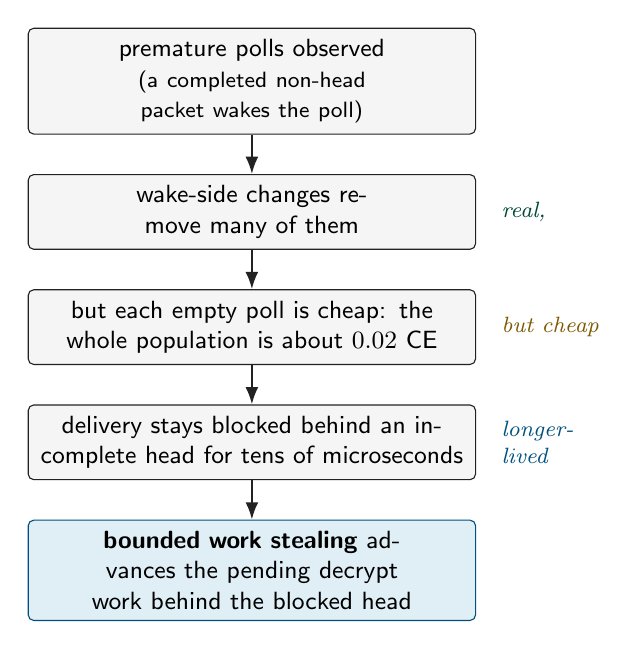
\begin{tikzpicture}[
  font=\sffamily\small,
  >={Latex[length=2.2mm]},
  node distance=5mm,
  fbox/.style={draw=cInk,rounded corners=2pt,align=center,text width=54mm,
               inner sep=4pt,minimum height=8mm,fill=black!4},
  goal/.style={draw=cBlue!70!black,rounded corners=2pt,align=center,text width=54mm,
               inner sep=4pt,minimum height=8mm,fill=cBlue!12},
  down/.style={->,thick,cInk},
  side/.style={font=\footnotesize\itshape,align=left}
]
\node[fbox] (s1) {premature polls observed\\{\footnotesize (a completed non-head packet wakes the poll)}};
\node[fbox,below=of s1] (s2) {wake-side changes remove many of them};
\node[fbox,below=of s2] (s3) {but each empty poll is cheap: the whole population is about $0.02$~CE};
\node[fbox,below=of s3] (s4) {delivery stays blocked behind an incomplete head for tens of microseconds};
\node[goal,below=of s4] (s5) {\textbf{bounded work stealing} advances the pending decrypt work behind the blocked head};

\draw[down] (s1) -- (s2);
\draw[down] (s2) -- (s3);
\draw[down] (s3) -- (s4);
\draw[down] (s4) -- (s5);

\node[side,anchor=west,text=cTeal!45!black] at ([xshift=2mm]s2.east) {real,};
\node[side,anchor=west,text=cAmber!55!black] at ([xshift=2mm]s3.east) {but cheap};
\node[side,anchor=west,text=cBlue!70!black] at ([xshift=2mm]s4.east) {longer-\\lived};

\end{tikzpicture}
\end{document}
